\documentclass[oneside]{book}

\usepackage{enumerate}% http://ctan.org/pkg/enumerate

% Pictures
\usepackage{graphicx}
\usepackage{grffile}
\usepackage{mwe}
\usepackage{subfig}


% Custom environments
\usepackage[english]{babel}
\usepackage{blindtext}
\usepackage{pifont,mdframed}
\usepackage[dvipsnames]{xcolor}

% graphics
\usepackage{tikz}
\usetikzlibrary{calc,patterns,angles,quotes}

% math
\usepackage{amsmath}
\usepackage{amsthm}

% SI units
\usepackage{siunitx}

% Make margins reasonable
\usepackage{fullpage}
\usepackage{changepage}   % for the adjustwidth environment

% Make TOC clickable
\usepackage{xcolor}
\usepackage{hyperref}

% Graphics
\usepackage{graphicx}
\graphicspath{
	{images/}
}


% References
\usepackage{fancyref}

% Index
\usepackage{mfirstuc}
\usepackage{makeidx}

% Header information
\title{Physics: Notes for Independent Learning}
\author{Jeffrey A. Robinson}

\makeindex
% Add index to TOC
\usepackage[totoc]{idxlayout}

%
%	Defined functions
%

% Theorem, Definitions, Proofts
\theoremstyle{definition}
\newtheorem{definition}{Definition}[chapter]

% Overline and under line text
\makeatletter
\newcommand*{\textoverline}[1]{$\overline{\hbox{#1}}\m@th$}
\makeatother

\makeatletter
\newcommand*{\textunderline}[1]{$\underline{\hbox{#1}}\m@th$}
\makeatother

\makeatletter
\newcommand*{\textbottomtopline}[1]{\textunderline{\textoverline{#1}}}
\makeatother

% Roman Numerals inline
\makeatletter
\newcommand*{\rom}[1]{\expandafter\@slowromancap\romannumeral #1@}
\makeatother


\newcommand{\force}[1]{#1~\si{\newton}}
\newcommand{\velocity}[1]{#1~\si{\meter/\second}}
\newcommand{\acceleration}[1]{#1~\si{\meter/\second^2}}
\newcommand{\mass}[1]{#1~\si{\kilo\gram^2}}
\newcommand{\distance}[1]{#1~\si{\meter}}
\newcommand{\seconds}[1]{#1~\si{\second}}
\newcommand{\hours}[1]{#1~\si{\hour}}

% Not SI
\newcommand{\lbs}[1]{#1~\si{lb}}

% format and add to index
\newcommand{\addindex}[1]{%
  \textbf{#1}%
  \index{#1@\protect\capitalisewords{#1}}%
   }
\makeatother

\newcommand{\vT}[2]{\left<#1,#2\right>}

% refs
\newcommand{\Def}[1]{Definition~\ref{#1}}
\newcommand{\Fig}[1]{Figure~\ref{#1}}
\newcommand{\Eq}[1]{Equation~\ref{#1}}

%
%	Defined Environments
%
\newenvironment{caution}
  {%
  	\par\begin{mdframed}%
		\begin{list}{}{									%
			\leftmargin=1cm								%
			\labelwidth=\leftmargin						%
		}\item[											%
			\color{BurntOrange}							%
        	\large\textsc{\textbottomtopline{Caution}}	%
        ]												%
  }
  {\end{list}\end{mdframed}\par}


\newcounter{DiscussionCounter}[chapter]
\newcounter{ExerciseCounter}[chapter]

\newcommand{\Before}[0]{}
\newcommand{\After}[0]{}

\newcommand{\discussion}[1]{%
	\noindent\begin{minipage}{\textwidth}%
		\noindent\stepcounter{DiscussionCounter}\textbf{Q\arabic{chapter}.\arabic{DiscussionCounter}}%
		\vspace{1mm}%
		\begin{adjustwidth}{0.5cm}{}\Before#1\After%
		\end{adjustwidth}%
		\vspace{5mm}%
	\end{minipage}
}

\newcommand{\exercise}[1] {
	\noindent\begin{minipage}{\textwidth}
		\noindent\stepcounter{ExerciseCounter}\textbf{\arabic{chapter}.\arabic{ExerciseCounter}}\vspace{1mm}
		\begin{adjustwidth}{0.5cm}{}\Before#1\After\end{adjustwidth}
	\end{minipage}\vspace{5mm}
}

\setcounter{secnumdepth}{0}

% Begin
\begin{document}

\frontmatter

% Title and TOC
\maketitle
\tableofcontents

\mainmatter


\chapter*{Preface}\addcontentsline{toc}{chapter}{Preface}

The purpose of this document is really as a reference for when someone needs to check their answer.  As there is no, as far as I can tell, steps involved I expect anyone who might look at this to use it to see if they get the same answer as I did.  I don't think every answer is correct so do be careful and triple check your work.




\part{Mechanics}

\chapter{Units, Physical Quantities, and Vectors}

\section{Notes}

The most important thing about this section is 
\begin{itemize}
	\item{Using the units to ensure that calculation are correctly performed.}
	\item{Estimating results to determine get a good feel on if your result makes sense.}
	\item{Error notation and their meaning. Mostly just to understand what you are reading.}
\end{itemize}

Understanding vectors is nice, but you should not spend more than a few minutes reading about them. In most cases you can "learn on the job". The only important things you need to know right now are,

\begin{itemize}
	\item{Vectors have a direction and a magnitude (length).}
	\item{Vectors are made of components; usually x, y, and z in Physics.}
	\item{In most cases vector components are independent of the component. For example, Up/Down don't impact left/right.}
\end{itemize}

\section{Discussion Questions}

% 1.1
\discussion{We just need a single experiment to disprove a theory.  However, there is no number of experiments to prove a theory, just increase confidence.  If there are only a finite number of possible outcomes this is obviously not true..}

% 1.2
\discussion{Two possible answers based on what they mean by tangent, 1) The tangent function takes in degrees and not distances. 2) The tangent of a line requires a function (or a continuous set of points) to compute a the tangent of a line.}

% 1.3
\discussion{My height in imperial is 6' 2", which is 187.96 cm.  My weight is 178 lbs in imperial and therefore it is 792.1 N}

% 1.4
\discussion{Yes.  Currently the mass is derived directly from these.  Other quantities are based off of properties events in nature, but the mass is derived by humans. As an aside, the mass increase is probably from oxidation or some similar process in which the reference mass is absorbing molecules or elements from the air.}

% 1.5
\discussion{You could use pulsars as a way to measure time as they have a very precise rotation.  Less precise measures could be position of sun in the sky to determine the hour of day.}

% 1.6
\discussion{Let's assume an 8 by 11 inch sheet of paper.  Then you can cut it into squares of 1x1 inch and then stack them up.  Measure that value and then divide it by 88 to approximate the thickness of a piece of paper. An alternative is to just fold it instead of cutting it up, but then you will not be able to get a more accurate answer.}

% 1.7
\discussion{An axiom is a self consistent statement.  It does not mean that it matches reality.  In terms of physics you could argue that an axiom is only true if the assumptions you are making are true.  A theory is only true as far as the experiments have shown it to be the best match based on observations.}

% 1.8
\discussion{The units of volume are meter-cubed and centimeter-cubed. The provided formula is "length" to the fourth, not the third as required.}

% 1.9
\discussion{Joe is not accurate but is precise, Moe is accurate but not precise, Flo is both accurate and precise.}

% 1.10
\discussion{No, the length of $(1,1,1)$ is $\sqrt{3}$.  No, the length of $(3,-2)$ is $\sqrt{11}$}

% 1.11
\discussion{Simple math, $\frac{9.8*60}{0.03^2} \approx{} 653KN/m$, $\frac{9.8*600}{0.092903} \approx{} 63KN/m$, over a 10x difference.}

% 1.12
\discussion{There are no two vectors with different lengths that when summed together are 0.  This is due to the fact of dimensional independence requires that to get 0 the entries in the vector as the same position must have the same magnitude but different sign.  To get three vectors of different lengths you can create three vectors of the form: $\vec{A} = (x,y,0), \vec{B} = (-x,0,z), \vec{C} = (0,-y,-z)$ where $|x| > |y| > |z|$. From here it is easy to show that $|\vec{A}| > |\vec{B}| > |\vec{C}|$.}

% 1.13
\discussion{The speed of light is 299,792,458 m/s and the radius of the earth is 6,400 km, or 6,400,000 m.  Therefore the circumference, 2$\pi{}$r, is 40,212,385.9659, then the circumference divided by the speed of light is 0.1341340814 seconds.}

% 1.14
\discussion{These are not vectors as they have no distance.}

% 1.15
\discussion{Only if dealing with imaginary numbers. Otherwise you will have a magnitude of $\sqrt{A^2 + B^2}$ and the only way that is zero is if A and B are both zero.  As before this would have to involve imaginary numbers.  You can do a proof to show that $\sqrt{\sum A_i^2} \geq |A_i| \forall i$}

% 1.16
\discussion{(a) No. (b) Only in reference to another vector, which points in the opposite direction.  Because all the component values of the two vectors are negatives of each other.  i.e $\vec{A}$ is the negative of $\vec{B}$ if-and-only-if $\forall i~A_i = -B_i$}

% 1.17
\discussion{For the first question $\vec{A}$ and $\vec{B}$ are multiples if each other. For the second question they both have to be the zero vector.}

% 1.18
\discussion{No.  Since neither are the zero vector when using the formulas $|\vec{A}| |\vec{B}| \cos{\alpha}$ and $|\vec{A} \times{} \vec{B}| = |\vec{A}||\vec{B}|\sin{\alpha}$ either $\sin{\alpha}$ or $\cos{\alpha}$ is 0 but not both.}

% 1.19
\discussion{No.  Time has a single component, and you can also do a 1:1 mapping to the reals (trivially) which is defined to be a scalar.}

% 1.20
\discussion{You can work out the math to show it is a unit vector, the direction is the same direction as $\vec{A}$.  Using the identify $\vec{A}/A \cdot \vec{i} = |\vec{A}/A||\vec{i}|cos{\left(\alpha\right)}$ then we have the right side just equal to $cos{\left(\alpha\right)}$.}

% 1.21
\discussion{The percent error is $1 - \frac{890010}{890000} = 1\mathrm{e}{-6}\%$.  You can argue in this case it is correct to display all digits as the exact distances are known.}

% 1.22
\discussion{Assuming 3-dim vectors, (a) Valid (b) Valid (c) Valid (d) Valid (e) No, cannot do cross product between Vector and scalar.}

% 1.23
\discussion{The cross product products a vector which is orthogonal to the original as long as not same vector.  You can just pick $\vec{A}$ and $\vec{B}$ to be the same.  If they are all zero obviously they are same.}

% 1.24
\discussion{Cross product produces vector orthogonal to original two.  The dot product of two orthogonal vectors is 0.}

% 1.25
\discussion{No.  $\vec{A} = (1,0,0)$ and $\vec{B} = (0,1,0)$ will satisfy this.}

% 1.26
% TODO : Figure out what they are asking.
\discussion{I don't know what they are talking about.  Their question makes no sense.}

\section{Exercises}

\subsection{Standard and Units, Using and Converting Units}

% 1.1
\exercise{ Some definitions: 1in = 2.54cm, 12in = 1ft, 5280ft = 1 mi, 2.54 * 5280 * 12 / 100000 = (a) 1.60 mi = 1.60 mi * 5280ft/mi =  2.57 km (b) 1.18 miles}

% 1.2
\exercise{28.9 in$^3$}

% 1.3
\exercise{$5.59\mathrm{e}{-9}$}

% 1.4
\exercise{13.5 g/cm$^3$ $\to$ 13.5$\mathrm{e}{3}$ kg/m$^3$ }

% 1.5
\exercise{5.36 L}

% 1.6
\exercise{6.86 Hectares}

% 1.7
\exercise{34.9 Years older}

% 1.8
\exercise{185000 furlong/fortnight $\cdot$ $\frac{1}{8}$ mi/furlong $\cdot$ $\frac{1}{14}$ fortnight/days $\cdot$ $\frac{1}{24}$ day/hour = 66.96428571 mi/hour $\approx$ 67.0 mi/hour.}

% 1.9
\exercise{(a) 23 \si{\kilo\meter/\liter} (b) 1.6 Tanks}

% 1.10
\exercise{(a) 88 ft/s (b) 9.754 \si{\meter/\second^2} (c) 1000 $\si{\kilo\gram/\meter^3}$}

% 1.11
\exercise{9.0 \si{\centi\meter}}

% 1.12
\exercise{(a) 4.10$\times$10$^8$ \si{\micro\gram/day}}

% 1.13
\exercise{(i) $\frac{32}{3}\times10^{-8}$ (ii) $8\pi\times10^{-6}\si{\milli\meter^2}$}

\subsection{Uncertainty and Significant Figures}

% 1.14
\exercise{(a) \num{96} \si{\milli\meter^2} (b) 0.37 (c) 43.96 \si{\milli\meter} (d) 10 \si{\milli\meter} (e) 2.7}

% 1.15
\exercise{$\approx{0.45\%}$}

% 1.16
\exercise{(a) 3.14236 (b) 3.14159 (c) a: No, b: Yes}

\subsection{Estimates and Orders of Magnitude}

% 1.17
\exercise{Height in \si{\centi\meter}}

% 1.18
\exercise{16,000}

% 1.19
\exercise{7.1 $\times$ $10^8$ blinks in a lifetime}

% 1.20
\exercise{(a) 17 $\times$ $10^3$ \si{\meter^3/year} (b) 32 \si{\meter}}

% 1.21
\exercise{Average height of a female is 161.8 \si{\centi\meter} tall, assume $\approx{30 \si{\centi\meter}}$ wide and assume wall is 1 \si{\centi\meter} thick.  $\approx{\$936,000}$.}

% 1.22
\exercise{Estimations: beats/min$\approx{90}$, lifetime$\approx{80 years}$ (a) 3.8 $\times$ $10^9$ beats in a lifetime. (b) 5.0 $\times$ $10^7$ gallons pumped in a lifetime.}

% 1.23
\exercise{Estimations: diameter$\approx{1 \si{\milli\meter}}$ 2.4 $\times$ $10^5$ drops in a bottle}

\subsection{Vectors and Vector Addition}

\begin{figure}[!ht]
    \centering
\begin{tikzpicture}[scale=0.1]
  \coordinate (origo) at (0,0);

  % Sheet  
  \draw[thin,gray!40] (-17,-17) (17,17);
  \draw[->] (0,0)--(-17,0) node (-x) [left]{};
  \draw[->] (0,0)--(17,0) node (x) [right]{$x$};
  \draw[<->] (0,-17)--(0,17) node (y) [above]{$y$};
  
  % Vectors
  \draw[blue,->,thick] (0,0) -- (70:15) %
  	coordinate (B) node[right, text width=5em] %
  	{$\boldsymbol{\vec{B} (15 \si{\meter})}$};
  	
  \draw[blue,->,thick] (0,0) -- (143:10) %
  	coordinate (D) node[left, text width=5em] %
  	{$\boldsymbol{\vec{D} (10 \si{\meter})}$};
  	
  \draw[blue,->,thick] (0,0) -- (205:12) %
	coordinate (C) node[left, text width=5em] %
  	{$\boldsymbol{\vec{C} (12 \si{\meter})}$};
  	
  \draw[blue,->,thick] (0,0) -- (270:8) %
  	coordinate (A) node[right, text width=5em] %
  	{$\boldsymbol{\vec{A} (8 \si{\meter})}$};
  	
  % Angles
  \pic %
  	[
  		draw,
  		<-,
  		"$\ang{30.0}$"scale=0.75,
  		angle eccentricity=1.5,
  		angle radius=1cm
  	] %
  	{angle = B--origo--y};
  	
  \pic %
  	[
  		draw,
  		<-,
  		"$\ang{53.0}$"scale=0.75,
  		angle eccentricity=1.5,
  		angle radius=0.5cm
  	] %
  	{angle = y--origo--D};
  	
  \pic %
  	[
  		draw,
  		<-,
  		"$\ang{25.0}$"scale=0.75,
  		angle eccentricity=1.5,
  		angle radius=0.75cm
  	] %
  	{angle = -x--origo--C};
\end{tikzpicture}
    \caption{Problem 1.24}
    \label{fig:Problem1.24}
\end{figure}

% 1.24
\exercise{Using \Fig{fig:Problem1.24}.  Doing this in my head. (a) Angle, maybe around \ang{30} (\ang{33}), Looks around 10\si{\meter} (9\si{\meter}) (b) Angle, maybe \ang{25} (\ang{20}) from the negative y-axis and probably 20 m (c) Same as a but angle is now from negative x-axis (d) Same as b but angle is now from positive y-axis.}

% 1.25
\exercise{Magnitude: 7.83 \si{\kilo\meter}, Angle: \ang{38}}

% 1.26
\exercise{$(230,-37)$ \si{\meter}, Mag: 230 \si{\meter}, Deg: \ang{350}}

\subsection{Components of Vectors}

% 1.27
\exercise{Using \Fig{fig:Problem1.24}. \\
\mbox{} \\
\begin{tabular}{l l l l l}
Vector & Magnitude & Angle & X & Y \\ \hline
A & 270 \si{\meter} & \ang{8}  &  0 \si{\meter}    & -8 \si{\meter}    \\
B & 60 \si{\meter}  & \ang{15} &  7.5  \si{\meter} &  13.0 \si{\meter} \\
C & 205 \si{\meter} & \ang{12} & -10.9 \si{\meter} & -5.07 \si{\meter} \\
D & 143 \si{\meter} & \ang{10} & -7.99 \si{\meter} &  6.02 \si{\meter}
\end{tabular}}

% 1.28
\exercise{(a) \ang{335} (b) \ang{20.7} (c) \ang{122} (d) \ang{226} }

% 1.29
\exercise{
\begin{tabular}{l l l l l}
	x     & y  & angle & mag \\ \hline
	-8.12 \si{\meter} & 13 \si{\meter} & \ang{122}   & 15.3 \si{\meter}
\end{tabular}
}

% 1.30
\exercise{
\begin{tabular}{l l l l}
	x     & y   & angle & mag \\ \hline
	-20 \si{\meter}	  & -24 \si{\meter} & \ang{230}	& 31 \si{\meter}
\end{tabular}}

% 1.31
\exercise{
\begin{tabular}{l l l l l}
	Vector & X & Y & Angle & Magnitude \\ \hline
	A+B	&  7.5 \si{\kilo\meter} &  5.00 \si{\kilo\meter} & \ang{33.6} &	9.01 \si{\kilo\meter} \\
	B+A	&  7.5 \si{\kilo\meter} &  5.00 \si{\kilo\meter} & \ang{33.6} &	9.01 \si{\kilo\meter} \\
	B-A	&  7.5 \si{\kilo\meter} &  21.0 \si{\kilo\meter} & \ang{70.3} & 22.3 \si{\kilo\meter} \\
	A-B	& -7.5 \si{\kilo\meter} & -21.0 \si{\kilo\meter} & \ang{70.3} & 22.3 \si{\kilo\meter}
\end{tabular}}

% 1.32
\exercise{Magnitude: 7.83 \si{\kilo\meter}, Angle: \ang{38}}

% 1.33
\exercise{
\begin{tabular}{l l l l}
	x    & y    & angle & mag \\ \hline
	1.95 \si{\kilo\meter} & -3.9  \si{\kilo\meter}& \ang{296} & 4.36 \si{\kilo\meter}
\end{tabular}}

% 1.34
\exercise{
\begin{tabular}{l l l l}
	x    & y    & angle & mag \\ \hline
	-8.60 \si{\centi\meter} &  5.20 \si{\centi\meter} & \ang{329}  & -10.0 \si{\centi\meter} \\
	-9.70 \si{\meter} & -2.45 \si{\meter} & \ang{14.2} & -10.0 \si{\meter} \\
	 7.75 \si{\kilo\meter} & -2.70 \si{\kilo\meter} & \ang{341}  &  8.21 \si{\kilo\meter}
\end{tabular}}


\begin{figure}[!ht]
    \centering
\begin{tikzpicture}[scale=0.7]
  \coordinate (origo) at (0,0);

  % Sheet  
  \draw[thin,gray!40] (-2,-2) (3,3);
  \draw[<->] (-2,0)--(3,0) node (x) [right]{$x$};
  \draw[<->] (0,-2)--(0,3) node (y) [above]{$y$};
  
  % Vectors
  \draw[blue,->,thick] (0,0) -- (60:2.8) %
  	coordinate (A) node[right, text width=5em] %
  	{$\boldsymbol{\vec{A}}~(2.8~\si{\centi\meter})$};%
  \draw[blue,->,thick] (0,0) -- (-60:1.90) %
  	coordinate (B) node[right, text width=5em] %
  	{$\boldsymbol{\vec{B}}~(1.9~\si{\centi\meter})$};%
% Angles
  \pic %
  	[
  		draw,
  		<->,
  		"$\ang{60.0}$"scale=0.75,
  		angle eccentricity=1.5,
  		angle radius=1cm
  	] %
  	{angle = x--origo--A};
  	
  \pic %
  	[
  		draw,
  		<->,
  		"$\ang{60.0}$"scale=0.75,
  		angle eccentricity=1.5,
  		angle radius=1cm
  	] %
  	{angle = B--origo--x};
\end{tikzpicture}
    \caption{Problem 1.35}
    \label{fig:Problem1.35}
\end{figure}


% 1.35
\exercise{Using \Fig{fig:Problem1.35}. \\
\mbox{} \\
\begin{tabular}{l l l l l}
    Vector &  Angle & Magnitude \si{\centi\meter} &  X \si{\centi\meter}   &  Y \si{\centi\meter}	 \\ \hline
    A+B    &  18.3  & 2.48      &  2.35 &  0.779 \\
    A-B    &  83.7  & 4.10      &  0.45 &  4.07  \\
    B-A    &  264   & 4.10      & -0.45 & -4.07
\end{tabular}}

\subsection{Unit Vectors}

% 1.36
\exercise{
\begin{tabular}{l l l}
	Part &  X    & Y     \\ \hline
	a    &  3.20 & -6.50 \\
	b    & -7.91 & 18.2  \\
	c    & -12   & 21.2  \\
	d    &  40   & -20
\end{tabular}}

% 1.37
\exercise{
\begin{tabular}{l l}
	Name & value  \\ \hline
	A    & $(0\hat{i} - 8\hat{j})$ \\
	B    & $(7.5\hat{i} + 13\hat{j})$ \\
	C    & $(-10.9\hat{i} - 5.07\hat{j})$ \\
	D    & $(-7.99\hat{i} + 6.02\hat{j})$
\end{tabular}}

\begin{figure}[!ht]
    \centering
\begin{tikzpicture}[scale=0.3]
  \coordinate (origo) at (0,0);

  % Sheet  
  \draw[thin,gray!40] (-1,-3) (8,10);
  \draw[<->] (-1,0)--(8,0) node (x) [right]{$x$};
  \draw[<->] (0,-3)--(0,10) node (y) [above]{$y$};
  
  % Vectors
  \draw[blue,->,thick] (0,0) -- (4,7) %
  	coordinate (A) node[right, text width=5em] %
  	{$\boldsymbol{\vec{A}}$};%
  \draw[blue,->,thick] (0,0) -- (5,-2) %
  	coordinate (B) node[right, text width=5em] %
  	{$\boldsymbol{\vec{B}}$};%
  \draw[blue,->,thick] (4,7) -- (-1,9) %
  	coordinate (T) node at (0,10) [right, text width=5em] %
  	{$\boldsymbol{\vec{T}}$};%
  \draw[blue,->,thick] (0,0) -- (-1,9) %
  	coordinate (A-B) node[left, text width=5em] %
  	{$\boldsymbol{\vec{A-B}}$};%
\end{tikzpicture}
    \caption{Problem 1.38}
    \label{fig:Problem1.38}
\end{figure}

% 1.38
\exercise{(a) $|\vec{A}| = $8.06 $|\vec{B}|$ = 5.39 (b) -$\hat{i} + 9\hat{j}$ (c) 9.06 \ang{96.3} (d) See \Fig{fig:Problem1.38}.
}


\begin{figure}[!ht]
    \centering
\begin{tikzpicture}[scale=0.7]
  \coordinate (origo) at (0,0);

  % Sheet  
  \draw[thin,gray!40] (-3,-3) (5,4);
  \draw[->] (0,0)--(-3,0) node (-x) [right]{};
  \draw[<->] (0,0)--(5,0) node (x) [right]{$x$};
  \draw[<->] (0,-3)--(0,4) node (y) [above]{$y$};
  
  % Vectors
  \draw[blue,->,thick] (0,0) -- (70:3.6) %
  	coordinate (A) node[right, text width=5em] %
  	{$\boldsymbol{\vec{A}}~3.6 m$};%
  \draw[blue,->,thick] (0,0) -- (210:2.4) %
  	coordinate (B) node[below, text width=5em] %
  	{$\boldsymbol{\vec{B}}~2.4 m$};%
% Angles
  \pic %
  	[
  		draw,
  		<->,
  		"$\ang{70.0}$"scale=0.75,
  		angle eccentricity=1.5,
  		angle radius=1cm
  	] %
  	{angle = x--origo--A};
  	
  \pic %
  	[
  		draw,
  		<->,
  		"$\ang{30.0}$"scale=0.75,
  		angle eccentricity=1.5,
  		angle radius=1cm
  	] %
  	{angle = -x--origo--B};
\end{tikzpicture}
    \caption{Problem 1.39}
    \label{fig:Problem1.39}
\end{figure}

% 1.39
\exercise{\Fig{fig:Problem1.39} as reference.  \\
(a) $\vec{A} = 2.08\hat{i}~\si{\meter} + 1.20\hat{j}~\si{\meter}$, $\vec{B} = -1.23\hat{i}~\si{\meter} - 3.38\hat{j}~\si{\meter}$ \\
(b) $\vec{C} = 11.2\hat{i}~\si{\meter} + 17.1\hat{j}~\si{\meter}$ \\
(c) 20.4~\si{\meter}}

% 1.40
\exercise{(a) \ang{153} (b) \ang{15.9} (c) \ang{63.4}}

% 1.41
\exercise{
(a) $|\vec{A}|=5.39$ $|\vec{B}|=4.369$ \\
(b) $\vec{A}-\vec{B} = -5\hat{i} + 2\hat{j} + 7\hat{k}$ \\
(c) $|\vec{A}-\vec{B}| = 8.83$. Opposite direction but same magnitude.
}

\subsection{Products of Vectors}

% 1.42
\exercise{\ang{82.1}}

% 1.43
\exercise{
(a) 104 (b) -148 (c) -40.6
}

% 1.44
\exercise{$(0,0,-43)$}

% 1.45
\exercise{
(a) \ang{165}
(b) \ang{28.1}
(c) \ang{90}
}

% 1.46
\exercise{ (a) mag: 4.61 dir: $(0,0,-1)$ (b) mag: 4.61 dir: $(0,0,1)$}

% 1.47
\exercise{(a) mag: 64.9 dir: $(0,0,-1)$ (b) mag: 63.9 dir: $(0,0,1)$}

% 1.48
\exercise{(a) -7.47 (b) mag: 4.33 dir: $(0,0,-1)$ }


\section{Problems}

\problem{
Common Stuff:
$Density=\frac{Mass}{Volume}$\\
Volume = $\frac{4}{3}\pi{}r^3$. \\


A) Earth Radius: 6.371*$10^{6}$m, Earth Mass: 5.972*$10^{24}$kg \\
Volume = = $\frac{4}{3}\pi{}(6.371*10^{6})^2$ \\
So the density is $\frac{3* 6.371}{4 * \pi * (5.972)^3} * \frac{10^{24}}{(10^6)^3}$ and Excel says this is equal to $5.51*10^3 kg/m^3$. I doubled checked online and it matches up. To convert to $g/cm^3$ just multiple by 1/1000 to get $5.51~g/cm^3$ \\


B) Sun Mass: $1.989*10^{30}$ \\
Density = $\frac{3 * 1.989}{4 * \pi * 255} * \frac{10^{30}}{10^{8}} = 1.41*10^{17}kg/m^3 = 1.41*10^{14}g/cm^3$. \\


C) Just the same formula for (B) but 20km and you get $1.78*10^{20} kg/m^3$ or $1.78*10^{17}g/cm^3$
}
\section{Challenge Problems}

\chapter{Motion along a Straight Line}

\section{Discussion Questions}

% 2.1
\discussion{Speed.  Velocity has a direction as well as a magnitude.}

% 2.2
\discussion{Since the dots appear to be increasing by what appears a multiple of the previous distance I would say it is graph (d).}

% 2.3
\discussion{Yes, if the velocity and acceleration have ``different signs''.  This is because the velocity is ``slowing down'' and will eventually reach zero, then start ``increasing again''.  You can also look at the formula for velocity with constant acceleration to see why.  It cannot reverse twice though as a straight line cannot pass through the x-axis twice.}

% 2.4
\discussion{Either when the velocity is constant or special cases when the acceleration changes direction and after a period of time the average velocity will match the instantaneous velocity.}

% 2.5
\discussion{ (b) Yes.  When the velocity and acceleration are in ``opposite directions''.  Yes, if they both point in the ``same direction''.}

% 2.6
\discussion{Constant acceleration.  Anytime you start from 0 speed and accelerate then end up at 0 speed will the speed equal the magnitude of the velocity at some point.}

% 2.7
\discussion{Average velocities are the same but in opposite directions.}

% 2.8
\discussion{You could argue that you would be able to ticket all parked cars that people who speed pass by.}

% 2.9
% This question is no very clear.  I assume they mean instantaneous velocity when they say velocity.
\discussion{No, because displacement is 0, $\Delta{x}$ = zero, then by definition the average velocity is 0.  For the second yes;  $x =sin(t)$, then $y=cos(t)$.  When t = 0 displacement is 0 but velocity is 1.}

% 2.10
\discussion{Yes. If you assume the object is already moving and there is no acceleration then the object will keep moving.}

% 2.11
\discussion{180km/hr * 1h/60m * 1m = 3km. 6.0 seconds is 1/10th of a minute, so 1/10th of 3km, 0.3km}

% 2.12
\discussion{360km/hr, since this is linear half the time means twice the speed.}

% 2.13
\discussion{(a) one being a straight line and the other being a parabola going throught the two points.  (b) Average V is $\delta{x}/\delta{t}$ so same for both.}

% 2.14
\discussion{No.  Imagine the top half of a circle starting a 0~\si{\meter/\second} and ending with 0~\si{\meter/\second}, the average would be 0, which it obviously isn't.}

% 2.15
\discussion{Thrown.  The distance travelled to go from 0 to the starting speed is more than the distance from your hand to the top.  If you calculate the acceleration you can see that in your hand is higher.}

% 2.16
\discussion{Your friend will beat you, it takes you $\frac{21}{20}~\si{\hour}$ and your friend $\frac{3}{5}~\si{\hour}$.}

% 2.17
\discussion{-9.8\si{\meter/\second^2}, it starts at that value but decreases over time.}

% 2.18
\discussion{The elevator.}

% 2.19
\discussion{(a) Same speed (b) Ball thrown down (c) Same (d) Ball thrown up }

% 2.20
\discussion{Less than 4~\si{\meter/\second}}

% 2.21
\discussion{Velocity is 0, and it is changing.  This change is the acceleration.}

% 2.22
\discussion{$\sqrt(3)T$}

\section{Exercises}

\subsection*{Displacement, Time, and Average Velocities}

% 2.1
\exercise{\distance{32.9}}

% 2.2
\exercise{
(a) \velocity{-0.00476} \\
(b) \velocity{0}
}

% 2.3
\exercise{1.38 hours longer}

% 2.4
\exercise{
(a) \velocity{4.4} \\
(b) \velocity{-7.3}}

% 2.5
\exercise{
(a) \velocity{0.28} \\
(b) \velocity{1.25}}

% 2.6
\exercise{
(a) \velocity{2.74} \\
(b) \velocity{4.94} \\
(c) \velocity{7.40}
}

\subsection*{Instantaneous Velocity}

% 2.7
\exercise{
(a) \velocity{41} \\
(b) v(0) = \velocity{21.8}, v(10) = \velocity{27}
}

% 2.8
\exercise{\velocity{3.62}}

% 2.9
\exercise{(a) $\frac{7}{3}$~\si{\meter/\second}, same for both (b) $V_{avg} = \frac{1}{3}$~\si{\meter/\second} $Speed_{avg} = \frac{7}{3}$~\si{\meter/\second} }

% 2.10
\exercise{(a) \rom{4} (b) \rom{1} (c) \rom{5} (d) \rom{2} (e) none }

% 2.11
\exercise{
A: \velocity{$\frac{20}{3}$} \\
B: \velocity{$\frac{20}{3}$} \\
C: \velocity{$0$} \\
D: \velocity{$-40$}
}

\subsection*{Average and Instantaneous Acceleration}

% 2.12
\exercise{
(a) (i) \acceleration{6} (ii) \acceleration{-6} (iii) \acceleration{0} (iv) \acceleration{0} \\
(b) \acceleration{0} and \acceleration{-6}
}

\begin{figure}[!ht]
    \centering
    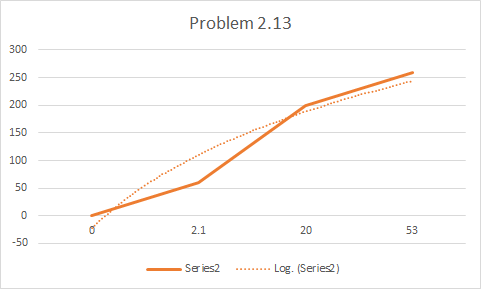
\includegraphics[scale=0.5]{mechanics/chapter2/problem2.13Speed.png}
    \caption{Problem 2.13}
    \label{fig:Problem2.13}
\end{figure}


% 2.13
\exercise{
(a) \Fig{fig:Problem2.13} \\
(b) (i) $\acceleration{28.6}$ (ii) $\acceleration{7.82}$ (iii) $\acceleration{1.82}$
}

% 2.14
\exercise{\acceleration{6.93}}

\begin{figure}[ht!]
    \begin{minipage}{.5\linewidth}
    \centering
    \subfloat[Position]{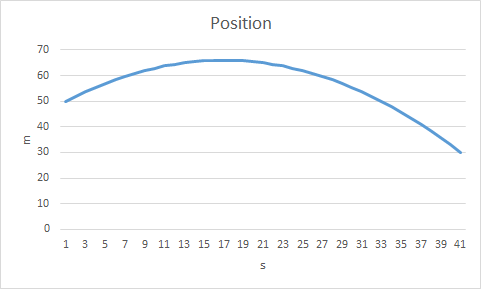
\includegraphics[scale=0.45]{mechanics/chapter2/problem2.15Position.png}\label{fig:Problem2.15Position}}
    \end{minipage}%
    \begin{minipage}{.5\linewidth}
    \centering
    \subfloat[Velocity]{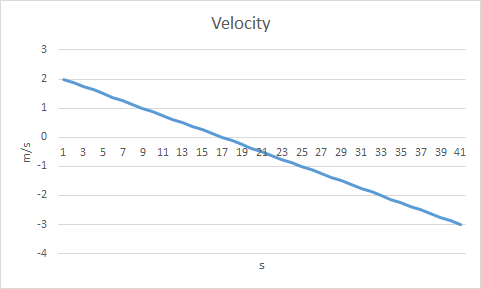
\includegraphics[scale=0.45]{mechanics/chapter2/problem2.15Velocity.png}\label{fig:Problem2.15Velocity}}
    \end{minipage}\par\medskip
    \centering
    \subfloat[Acceleration]{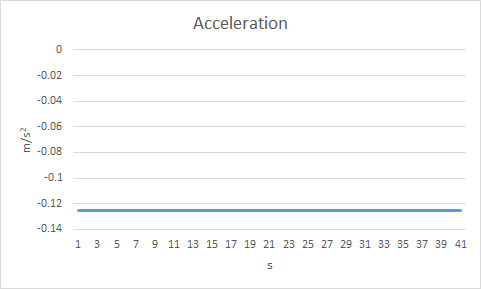
\includegraphics[scale=0.45]{mechanics/chapter2/problem2.15Acceleration.png}\label{fig:Problem2.15Acceleration}}

    \caption{Problem 2.15}
    \label{fig:Problem2.15}
\end{figure}

% 2.15
\exercise{(a) 2.00~\si{\centi\meter/\second} 50.0~\si{\centi\meter} 0.125~\si{\centi\meter/\second^2} \\
(b) \seconds{16} \\
(c) \seconds{32} \\
(d) \seconds{-13.9} and \seconds{45.9} \\
(e) \Fig{fig:Problem2.15}
}

% 2.16
\exercise{
(a) mag: \acceleration{0.963} sign: positive dir: right \\
(b) mag: \acceleration{0.963} sign: negative dir: left  \\
(c) mag: \acceleration{2.83} sign: negative dir: left
}

\begin{figure}[ht!]
    \begin{minipage}{.5\linewidth}
        \centering
        \subfloat[Position]{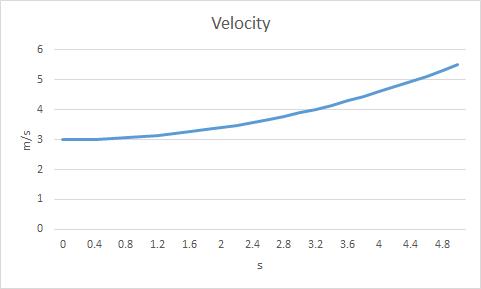
\includegraphics[scale=0.45]{mechanics/chapter2/problem2.17Velocity.png}\label{fig:Problem2.17Velocity}}
    \end{minipage}%
    \begin{minipage}{.5\linewidth}
        \centering
        \subfloat[Velocity]{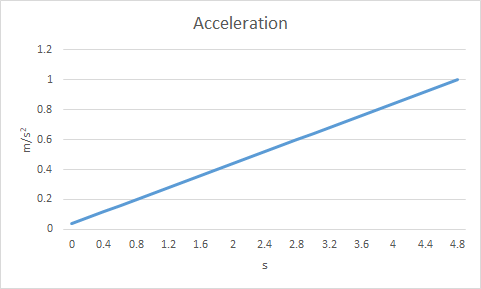
\includegraphics[scale=0.45]{mechanics/chapter2/problem2.17Acceleration.png}\label{fig:Problem2.17Acceleration}}
    \end{minipage}\par\medskip

    \caption{Problem 2.17}
    \label{fig:Problem2.17}
\end{figure}

% 2.17
\exercise{ 
(a) $0.5~\acceleration$ (b) \Fig{fig:Problem2.17}
}

\begin{figure}[ht!]
    \begin{minipage}{.5\linewidth}
    \centering
    \subfloat[Position]{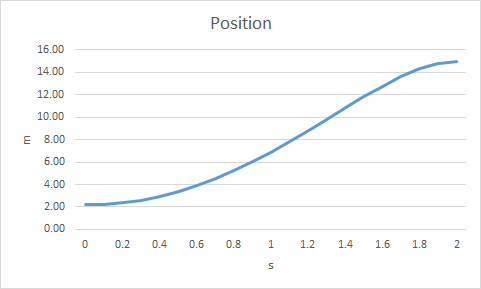
\includegraphics[scale=0.45]{mechanics/chapter2/problem2.18Position.png}\label{fig:Problem2.18Position}}
    \end{minipage}%
    \begin{minipage}{.5\linewidth}
    \centering
    \subfloat[Velocity]{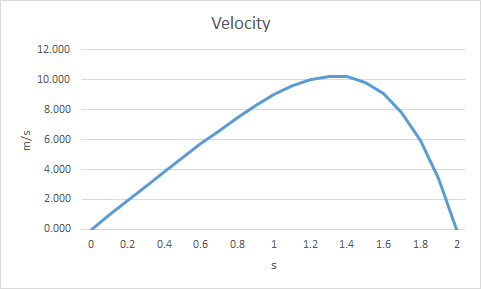
\includegraphics[scale=0.45]{mechanics/chapter2/problem2.18Velocity.png}\label{fig:Problem2.18Velocity}}
    \end{minipage}\par\medskip
    \centering
    \subfloat[Acceleration]{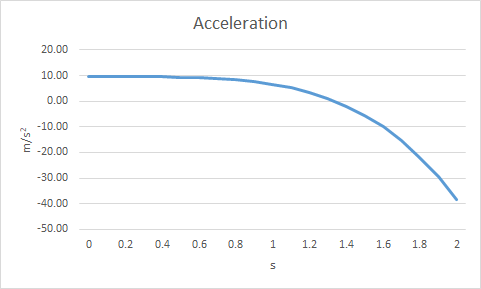
\includegraphics[scale=0.45]{mechanics/chapter2/problem2.18Acceleration.png}\label{fig:Problem2.18Acceleration}}

    \caption{Problem 2.18}
    \label{fig:Problem2.18}
\end{figure}

% 2.18
\exercise{
(a) t = 0 x = \distance{2.17}, t=+2 x = \distance{15}, t=-2 x = \distance{15} \\
(b) \Fig{fig:Problem2.18}
}

\subsection*{Motion with constant Acceleration}

% 2.19
\exercise{
(a) \velocity{5.40} \\
(b) \acceleration{1.36}
}

% 2.20
\exercise{
(a) Yes \\
(b) \velocity{245}
}

% 2.21
\exercise{\acceleration{736}}

% 2.22
\exercise{
(a) \acceleration{2500} \\
(b) \distance{1.06}
}

% 2.23
\exercise{\distance{1.55}}

% 2.24
\exercise{
(a) \seconds{33.8} \\
(b) \distance{662}
}

% 2.25
\exercise{\distance{0.38}}

% 2.26
\exercise{
(a) \acceleration{-39} \\
(b) \seconds{0.018}
}

% 2.27
\exercise{
(a) \acceleration{3.13e6} \\
(b) \seconds{0.016} \\
(c) No
}

% 2.28
\exercise{
(a) \velocity{1.4} \\
(b) \seconds{13} \\
(c) \distance{234}
}

% 2.29
\exercise{
(a) (i) 7.11e4\si{\kilo\meter/\hour^2} (ii) 9.84e4\si{\kilo\meter/\hour^2} \\
(b) (i) 0.18~\si{\kilo\meter} (ii) 13~\si{\kilo\meter}
}

% 2.30
\exercise{
(a) 1.7\si{\centi\meter/\second} \\
(b) 1.4\si{\centi\meter/\second} \\
(c) TODO: Take picture
}

% 2.31
\exercise{
(a) \acceleration{7.5}, \acceleration{12.5} \\
(b) \distance{400}, \distance{195}, \distance{285}
}

% 2.32
\exercise{
TODO: Do and take picture of resulting graphs.
}

% 2.33
\exercise{
$V_f$ = \velocity{2.68}
}

% 2.34
\exercise{
(a) \distance{246} \\
(b) \velocity{41.1} \\
(c) TODO: Take picture \\
(d) TODO: Take picture
}

\subsection*{Freely Falling Bodies}

% 2.35
\exercise{
$v = \sqrt{2g\Delta{x}}$, $t = 2\Delta{x}/(V_0+V_f)$ \\
(a) \velocity{4.6} \\
(b) \seconds{0.116}
}

% 2.36
\exercise{
   (a) \velocity{32.4} \\
   (b) \seconds{1.47}
}

% 2.37
\exercise{
    \seconds{1.65}
}

% 2.38
\exercise{
	(a) \velocity{4.11} \\
	(b) \seconds{0.468}
}

% 2.39
\exercise{
	(a) \distance{26.0} \\
	(b) \velocity{13.9} \\
	(c) TODO
}

% 2.40
\exercise{
	\velocity{-4.1}
}

% 2.41
\exercise{
	(a) $t = \sqrt{2\Delta{X}/a}$ \\
	(b) \seconds{0.059}
}

% 2.42
\exercise{
	(a) \distance{17.7} \\
	(b) \velocity{18.6} \\
	(c) TODO
}

% 2.43
\exercise{
	(a) \distance{678} \\
	(b) \seconds{11} \\
	(c) TODO
}

% 2.44
\exercise{
	(a) x(0.155) = \distance{0.66}, x(1.20) = \distance{-1.06} \\
	(b) \seconds{23} \\
	(c) \velocity{-220} \\
	(d) \distance{41m} \\
	(e) TODO
}

% 2.45
\exercise{
	(a) \acceleration{250} \\
	(b) 25.5 \\
	(c) \distance{21} \\
	(d) No, only 21g
}

% 2.46
\exercise{
	(a) \velocity{17.1} \\
	(b) \distance{14.9} \\
	(c) \velocity{0} \\
	(d) \acceleration{-9.8} \\
	(e) TODO
}

% 2.47
\exercise{
	\velocity{0.0868}
}

% 2.48
\exercise{
	(a) \seconds{2.03} \\
	(b) \seconds{6.21} \\
	(c) \seconds{0} and \seconds{8.24} \\
	(d) \seconds{4.12} \\
	(e) All are \acceleration{-9.8} \\
	(f) TODO
}

% 2.49
\exercise{
	$V_f = \velocity{17.8}$
}

% 2.50
\exercise{
	\distance{47.3}
}

% 2.51
\exercise{
	(a) \distance{500} \\
	(b) \velocity{103} 
}

% 2.52
\exercise{
	(a) \velocity{689} \\
	(b) \distance{11.5} \\
	(c) TODO
}

% 2.53
\exercise{
	(a) $a(t) = At - Bt^2$, $v(t) = \frac{At^2}{2} - \frac{Bt^3}{3}$, $x(t) = \frac{At^3}{6} - \frac{12}{Bt^4}$ \\ 
	(b)\velocity{39.1}
}

% 2.54
\exercise{
	REDO
}

\section{Problems}

\section{Challenge Problems}

\chapter{Motion in Two or Three Dimensions}

\section{Discussion Questions}

% 3.1
\discussion{As there is no velocity at the end of the swing the only force acting on the pendulum is gravity. A the midpoint the only, acceleraton would be towards the ``center'' of the rope.}

% 3.2
\discussion{It turns, the speed would initially increase as the vectors are orthogonal.}

% 3.3
\discussion{Never parallel, perpendicular at the top.}

% 3.4
\discussion{
(a) Stays the same (unless floor curves) \\
(b) Twice the distance \\
(c) Same
}

% 3.5
\discussion{Same as $\Delta{\vec{x}}$ is same, total distance is not same.}

% 3.6
\discussion{Hit at the same time, thrown will have greater speed.}

% 3.7
\discussion{Unclear what they are asking.}

% 3.8
\discussion{Problem is not stated very clearly, assume $v_x = v_y$. $\Delta{y} = \frac{1}{2}\frac{v_0^2}{g}$}

% 3.9
\discussion{
$\vec{v} = \left<v_{0_x},0\right>$, speed = $v_{0_x}$, $\vec{a} = \acceleration{\left<0, -9.8\right> }$
}

% 3.10
\discussion{Average velocity and average acceleration is 0.}

% 3.11
\discussion{$\sqrt{2}\cdot{}10$}

% 3.12
\discussion{$\vec{v}(t) = \velocity{\left<10,10*t\right>}$, $\vec{v}(5) = \velocity{51}$, $\Delta{x} = \distance{123}$}

% 3.13
\discussion{The car is moving forward, therefore the raindrops ``smear'' against the window.  For the windshield it would require the wind as only the vertical streaks would form. The best mathematical explanation I can think of is that the ``smears'' appear when the raindrop and car velocities are not parallel.}

% 3.14
\discussion{TODO: Review.  The dot product of the velocities of the wind and rain.}

% 3.15
\discussion{Straight across if you just want to be on the other side.  If you want to be directly across from the spot you are you would need to swim at an angle against the flow of the river.}

% 3.16
\discussion{It would be (d).  It would start slowing down, then hit it's maximum height and the speed would be equal to $v_{0_x}$, then the speed would start increasing as gravity pulls it downward.}

\section{Exercises}

\subsubsection*{Position and Velocity Vectors}
% 3.1
\exercise{
(a) $\velocity{\vT{1.5}{1.2}}$ \\
(b) \velocity{1.9} $\ang{-39}$
}

% 3.2
\exercise{
(a) $\distance{\vT{-50}{54}}$ \\
(b) $\distance{74}$
}

\begin{figure}[!ht]
    \centering
    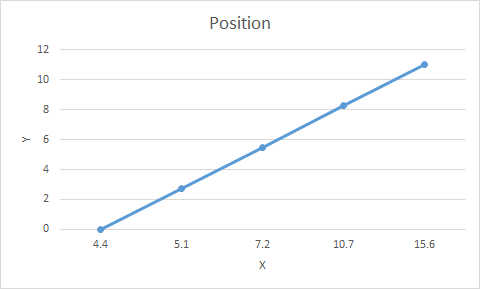
\includegraphics[scale=0.5]{mechanics/chapter3/problem3.3.png}
    \caption{Problem 3.3}
    \label{fig:Problem3.3}
\end{figure}

% 3.3
\exercise{
(a) $\acceleration{\vT{5.6}{5.5}}$ \\
(b) $\vec{v}(0) = \velocity{\vT{0.0}{5.5}}$, $\vec{v}(1) = \velocity{\vT{5.6}{5.5}}$, $\vec{v}(2) = \velocity{\vT{11.2}{5.5}}$ \\
(c) $\Fig{fig:Problem3.3}$ shows the position over time.
}

% 3.4
\exercise{
(a) $\vec{v}(t) = \velocity{\vT{0.280}{0.057t^2}}$ \\
(b) $\distance{4.26}$ \\
(c) $\velocity{1.88}, \ang{87.9}$
}

\subsubsection*{The Acceleration Vector}

\begin{figure}[!ht]
    \centering
    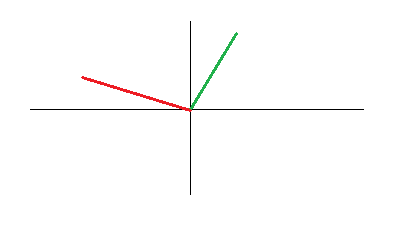
\includegraphics[scale=0.5]{mechanics/chapter3/problem3.5.png}
    \caption{Problem 3.5}
    \label{fig:Problem3.5}
\end{figure}

% 3.5
\exercise{
(a) $\Fig{fig:Problem3.5}$ \\
(b) $\acceleration{\vT{-8.77}{-2.67}}$ \\
(c) $\acceleration{9.16}, \ang{197}$
}

\begin{figure}[!ht]
    \centering
    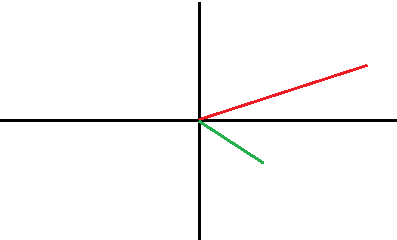
\includegraphics[scale=0.5]{mechanics/chapter3/problem3.6.png}
    \caption{Problem 3.6}
    \label{fig:Problem3.6}
\end{figure}


% 3.6
\exercise{
(a) $\velocity{\vT{}9.46{2.34}}$ \\
(b) $\velocity{9.74}, \ang{13.9}$ \\
(c) $\Fig{fig:Problem3.6}$
}

% 3.7
\exercise{
(a)TODO: Excel \\
(b) $\vec{v}(t) = \velocity{\vT{\alpha}{-2\beta{t}}}, \vec{a}(t) = \acceleration{\vT{0}{-2\beta}}$ \\
(c) $\vec{v}(2) = \velocity{\vT{2.4}{-4.8}}, \vec{a}(2)= \vT{0}{-2.4}$ \\
(d) TODO: Excel, Increasing, turning right
}

% 3.8
\exercise{
(a) $\vec{a}(t) = \acceleration{\vT{-0.036t}{0.550}}$ \\
(b) $\velocity{7.11}, \ang{35.7}$ \\
(c) $\acceleration{0.60}, \ang{336}$
}

\subsubsection{Projectile Motion}

% 3.9
\exercise{
(a) $\distance{0.502}$ \\
(a) $\distance{0.448}$ \\
(a) $\velocity{1.40}{-3.14}$ \\
(d) TODO
}

% 3.10
\exercise{$\velocity{1.30}$}

% 3.11
\exercise{\si{\centi\meter}}

% 3.12
\exercise{
(a) $\seconds{1.730}$ \\
(b) $\distance{14.7}$ \\
(c) $\seconds{1.73}$ \\
(d) $\distance{74.4}$ \\
(e) TODO
}

% 3.13
\exercise{
(a) $\velocity{28.6}$ \\
(b) $\velocity{34.6}$
}

% 3.14
\exercise{
(a) $\velocity{\vT{2.12}{3.3}}$ \\
(b) $\distance{7.34}$
}

% 3.15
\exercise{
$\acceleration{72.5}$
}

% 3.16
\exercise{
(a) $\velocity{\vT{39.8}{58.8}}$ \\
(b) $\seconds{6}$ \\
(c) $\distance{176}$ \\
(d) $\distance{239}$ \\
(e) $\vec{a_h} = \acceleration{\vT{0,-9.8}}$, $\vec{v_h} = \acceleration{\vT{39.8,}}$
}

% 3.17
\exercise{
(a) $t = \seconds{1.22}, \seconds{7.14}$ \\
(b) $\vec{v}(1.22) = \velocity{\vT{31.5}{8.54}}, \vec{v}(7.14) = \velocity{\vT{31.5}{-8.54}}$ \\
(a) $\velocity{33.0}, \ang{-38.5}$
}

% 3.18
\exercise{
(a) $\vec{a} = \acceleration{\vT{0}{-8.97}}$ \\
(b) $\vec{v_0} = \velocity{\vT{7.55}{9.33}}, \vec{v_f} = \velocity{\vT{7.55}{-9.33}}$ \\
(c) $\distance{15.7}$ \\
(d) Because g is a fixed value, it should be the current acceleration. \\
(e) TODO
}

% 3.19
\exercise{
(a)  $D = \distance{1.53}$ \\
(b)  $V = \velocity{-0.886}$
}

% 3.20
\exercise{
(a) $\ang{53.1}$ \\
(b) $\vec{a} \ \acceleration{\vT{0}{-9.8}}, \vec{v} \ \velocity{\vT{16}{0}}$ \\
(c) $\distance{15.9}$, $\velocity{18.6}$
}

% 3.21
\exercise{
(a) $\distance{12.9}$ \\
(b) $\distance{29.0}$ \\
(c) $\distance{39.3}$ \\
(d) TODO
}

% 3.22
\exercise{
(a) $\distance{288}$  \\
(b) $\distance{90.4}$ \\
(c) $\distance{90.4}$ \\
(b) $\vec{v_B} = \velocity{\vT{19.6}{-74.5}}, \vec{v_G} = \velocity{\vT{19.6}{100}}$
}

\subsubsection*{Motion in a Circle}

% 3.23
\exercise{
(a) $\acceleration{0.0337}, 0.00344$ \\
(b) $\hours{1.41}$
}

% 3.24
\exercise{$\acceleration{21.6}$}

% 3.25
\exercise{$\velocity{130}$}

% 3.26
\exercise{
(a) $\velocity{11.8}$ \\
(b) 9.47g
}

% 3.27
\exercise{
This problem seems to be ignoring gravity, or I don't understand something. Even an online article~\footnote{https://www.real-world-physics-problems.com/ferris-wheel-physics.html} says different. \\
(a) $\acceleration{3.63}$ upwards\\
(b) $\acceleration{3.63}$ downwards\\
(c) $\seconds{12.3}$
}

% 3.28
\exercise{
(a) $\velocity{2.98\cdot{}10^3}$ \\
(b) $\acceleration{5.95\cdot{}10^{-3}}$ \\
(c) $\velocity{4.78\cdot{}10^4}$, $\acceleration{3.95\cdots{}10^{-2}}$
}

% 3.29
\exercise{
(a) 12.5g   \\
(b) 2.83g   \\
(c) 255.5 rev/min
}

\subsubsection*{Relative Velocity}

% 3.30
\exercise{
(a) $\velocity{5.0}$ \\
(a) $\velocity{-16.0}$ \\
(a) $\velocity{-13.0}$
}

% 3.31
\exercise{
(a) $\seconds{10}$ \\
(b) $\seconds{110}$
}

% 3.32
\exercise{
 (4) $\seconds{2.75}$ \\
 (2.8) $\seconds{3.86}$
 
}

% 3.33
\exercise{$\velocity{0.42}, \ang{43}$
}

% 3.34
\exercise{TODO}

% 3.35
\exercise{
(a) $\velocity{4.9}, \ang{-16}$ \\
(b)$\seconds{210}$ \\
(c) $\distance{540}$
}

% 3.36
\exercise{
(a) $\velocity{\vT{4.2}{2.5}}$ \\
(b) $\velocity{4.9}, \ang{16}$ \\
(c) $\seconds{210}$
}

% 3.37
\exercise{
(a) $\ang{-120}$ \\
(b) $\hours{6.25}$
}

% 3.38
\exercise{
(a) $\ang{167}$ \\
(b) TODO
}

\section{Problems}

\section{Challenge Problems}


\chapter{Newton's Laws of Motion}

\section{Discussion Questions}

% 4.1
\discussion{A non-inertial frame is one in which Newton's first law does not hold.  Example given in book is roller-skater on a bus.  The second and third law should hold.}

% 4.2
\discussion{no air-resistance.}

% 4.3
\discussion{Because they don't have any force acting on those parts of the body so they don't start moving until they tense up or the seat hits them.}

% 4.4
\discussion{no acceleration so no force.}

% 4.5
\discussion{Because gravity is also at play.}

% 4.6
\discussion{It goes in a straight line target to circle at point let go. Eventually falls to the ground due to gravity.}

% 4.7
\discussion{Same as Q4.3,  They want to stay at the current velocity but car is acceleration.}

% 4.8
\discussion{Those are not forces.  Really describing velocity and Newton's first law.}

% 4.9
\discussion{Bus is accelerating or is on a hill.  There is no way to tell which.  }

% 4.10
\discussion{$N * s^2/m$}

% 4.11
\discussion{Earth is rotating on axis which is also rotating around sun which is rotating inside galaxy.}

% 4.12
\discussion{Yes.  The person will feel a force.}

% 4.13
\discussion{No, this is the result of the force.}

% 4.14
\discussion{$\acceleration{9.8}$}

% 4.15
\discussion{No, the ball will want to keep going in the same direction (relative to earth) and will appear to curve to the players.}

% 4.16
\discussion{Force is in newtons and the units don't match.  Also, the force of gravity is not technically constant.}

% 4.17
\discussion{
	(i) By Newton's second and third law.  The mass of the rock is much larger than that of you foot.  Therefore the acceleration your foot feels will be much higher than the rock.  \\
	(ii) No, you can remove the pain if you were to wear a shoe then the acceleration would be less, and also there would be cushion.
}

% 4.18
\discussion{Imagine jumping off a couch.  You crouch when you land with an acceleration away from the ground which is a small applied force over time.  Now imaging when you jump of a roof, you would need to accelerate much faster, so a larger force.}

% 4.19
\discussion{When jumping into water the water ``gives'' as you hit.  In essence you are applying a much smaller force over a longer period of time.  When you hit the earth you can't spread out the force on your body so you break your legs.}

% 4.20
\discussion{The affects of gravity become less influential.}

% 4.21
\discussion{When you double the amount of time the acceleration is $\frac{1}{4}^{th}$ the value.  This is not enough force to break the bonds on the string.}

% 4.22
\discussion{No, only if the same direction.}

% 4.23
\discussion{The stone with more mass.  Imagine you split the heavy stone in half, so you have two stones which each are the same mass as the first.  You then hold all three up at the same level and let go.  All three will hit the ground at the same time.  What is the difference between the stones being connected vs. being unconnected?  Nothing.  Also, you can think of gravity pulling on more stone, but at the same ``acceleration''.}

% 4.24
\discussion{kg is a mass, lb is a force.}

% 4.25
\discussion{The friction between the horse and the ground is much higher than the friction between the wagon and the ground.  Because of that the horse is moving forward and taking the wagon with it.}

% 4.26
\discussion{False.  Newton's third law.}

% 4.27
\discussion{The forces will be the same.  The accelerations on the other hand will not be.}

% 4.28
\discussion{
	(i) Friction from the road, engine, and other car components along with air resistance slows a car down. \\
	(ii)  Chemcial reactions are causing small explosions which are creating a force in the engine which is, inefficiently, transmitted to the wheel which then use the frictional force to accelerate the car.
}

% 4.29
\discussion{The force between the van and car are the same due to Newton's third law.  The total forces on the van would be larger than that on the car.  If we look at it as a closed system and the acceleration is the same on both vehicles then the force on the car has to be smaller as the mass is smaller than that of the van.}

% 4.30
\discussion{The force on the rope is the same but the friction on the ground for the two groups is not.  The weight of the groups matters as well as the strength of the occupants (hold rope, push against ground).}

% 4.31
\discussion{Less, $\force{100}$ be on the entire system. If we only look at each box then we see that the box with more ``weight'' has a higher force acting on it.}

% 4.32
\discussion{Does not sound like it.  Since the velocity appears to be constant the acceleration would be 0.}

% 4.33
\discussion{The water travels down your finger and flies off.  Also, the force from your hands  }

% 4.34
\discussion{the blood requires a force to move it up, but because blood is a liquid it can flow easier than a solid.  The blood is pushed by the veins and arteries and the blood pushes back as well.  The veins and arteries expand because of this push back so not all the blood moves up with you.}

% 4.35
\discussion{When the car is hit from behind you are pushed hard forward (Force) and then when you hit the seatbelt it pulls hard on your body (Force) but your head keeps going since it is on your neck but eventually your head will be pulled back by your neck and then you will start moving back into the seat.}

% 4.36
\discussion{With no seatbelt you will have no force acting on your body as the car stops.  Then you will hit the windshield (or steering wheel) and then have a force acting on your head.  If you have enough velocity you can make it through the windshield and then you will be stopped by either the car in front of you are the ground.}

% 4.37
\discussion{Same force because of Newton's third law.  Compact car has greatest acceleration due to Newton's Second law.  Therefore the occupants will have a larger acceleration acting on them compared to the larger vehicle, and therefore larger force.}

% 4.38
\discussion{
	(a) Can't \\
	(b) You would move towards the end of a rocket.
}

\section{Exercises}

\subsection{Force and Interactions}

% 4.1
\exercise{
	553N @ $\ang{27.2}$	
}

% 4.2
\exercise{
	866N @ $\ang{78.1}$	
}

% 4.3
\exercise{
	T = $\force{3.15}$
}

% 4.4
\exercise{
	(a) $\force{108}$ \\
	(b) $\force{54}$
}

% 4.5
\exercise{
	$\force{\vT{-6.69,2.83}}$, $\force{7.26} @ \ang{157}$
}

% 4.6
\exercise{
	(a) a = $\acceleration{2.5x10^{14}}$ \\
	(b) t = $\seconds{9.11x10^{-8}}$ \\
	(c) F = $\force{2.28x10^{-16}}$
}

% 4.7
\exercise{
	F = $\force{-46}$, $U_k = 0.0685$
}

% 4.8
\exercise{
	(a) $\force{822}$ \\
	(b) $\force{44.9}$
}

% 4.9
\exercise{
	$\mass{13.9}$
}

% 4.10
\exercise{
	(a) $\mass{90.9}$ \\
	(b) $\distance{22}$
}

% 4.11
\exercise{
	(a) x = $\distance{3.12}$, v = $\velocity{3.12}$ \\
	(b) x = $\distance{21.8}$, v = $\velocity{6.24}$
}

% 4.12
\exercise{
	(a) $a = \acceleration{4.38}$ \\
	(b) $x = \distance{370}$ \\
	(c) $v = \velocity{56.9}$
}

% 4.13
\exercise{
	(a) $Maximum force is\force{45.0}$, and it occurs between t = $\seconds{2} and \seconds{4}$ \\
	(b) Constant force from t = $\seconds{2} to \seconds{4}$ \\
	(c) At t = $\seconds{0} and \seconds{6}$
}

% 4.14
\exercise{
	(a) max force = $\force{45.0}$, from $\seconds{0} to \seconds{2}$ \\
	(b) from $\seconds{2} to \seconds{6}$ \\
	(c) Force @ $\seconds{8.5}$ is $\force{3.89}$
}

% 4.15
\exercise{
	(a) A = $\force{130.0}$, B = $\SI{5.5}{\newton/\second}$ \\
	(b) (i) $\force{81}, \acceleration{16.2}$,  (ii) $\force{148}, \acceleration{2.97}$ \\
	(c) $\acceleration{39.2}$
}

% 4.16
\exercise{
	(a) a =  $\acceleration{2.22}$ \\
	(b) m = $\mass{1.78}$
}

% 4.17
\exercise{
	F = $\force{2290}$
}

% 4.18
\exercise{
	(a) w(flea) = $\force{3.55}$ \\
	(b) w(frog) = $\force{1.21x10^{-1}}$ \\
	(c) w(cat) = $\force{4.4}$, $\lbs{9.71}$
}

% 4.19
\exercise{
	(a) $\mass{4.90}$ \\
	(b) $\force{8.87}$
}

% 4.20
\exercise{
	$force{1490}$
}

% 4.21
\exercise{
	(i) $\force{680}$ \\
	(ii) Equal and opposite forces.  The energy is stored in the body.
}

% 4.22
\exercise{
	Is accelerating at $\acceleration{-0.45}$
}

% 4.23
\exercise{
	$\force{24}$
}

% 4.24
\exercise{
	$\acceleration{7.7x10^-{24}}$
}

% 4.25
\exercise{
	(a) TODO: Excel \\
	(b) Yes.  The sum of the weights is non-zero.  The vertical components, gravity and the normal force, add to zero, however the horizontal forces add up to $\vec{F}$
}

% 4.26
\exercise{
	(a) TODO: Take picture \\
	(b) TODO: Take picture
}

% 4.27
\exercise{
	(a) TODO: Take picture, No net force. \\
	(b) TODO: Take picture, No net force from observer in vehicle, is one relative to earth.  Non-inertial frame.
}

% 4.28
\exercise{
	(a) t = $\seconds{7.43x10^{-4}}$ \\
	(b) F = $\force{-848}$
}

% 4.29
\exercise{
	$\force{154}$	
}


\section{Problems}

\section{Challenge Problems}


\chapter{Applying Newton's Laws}

\section{Discussion Questions}

% 5.1
\discussion{
	The tension (T) is the combined weight of the man and seat.  On each end of the rope there is a force equal to half the tension.
}

% 5.2
\discussion{
	If the only forces are the normal force and gravity then they are only equal if the ground you stand on is perfectly flat.  Two times they are not equal is when you are standing on a hill and when an elevator first starts moving.  When they are equal is when you are standing in an elevator not moving and when you are sitting down.
}

% 5.3
\discussion{
	The force of gravity pulls the rope down.  If there was no sag then that means a force is counter acting gravity.  If the string is straight then the poles have no force in the y direction to counter balance the force of gravity.  Since the only forces come from gravity and the poles there is no way that the rope can be perfectly flat.
}

% 5.4
\discussion{
	The external forces are: gravity, normal force, friction between tires and ground, and wind resistance. 
}

% 5.5
\discussion{
	(1) Have a device which pushes you at a set acceleration into a scale. \\
	(2) Attach pole to a spring, then have astronaut spin at end of pole for a set radial velocity that causes acceleration to be the same as earths. \\
	(3) Similar to \#2, spin a room so that it mimics gravity, then stand on scale.
}

% 5.6
\discussion{
	Pushing horizontal.  Because some of the force is being transfered into the ramp, which is then pushing back at you.
}

% 5.7
\discussion{
	It is falling at $\acceleration{9.8}$.  She is probably going to die.
}

% 5.8
\discussion{
	Down the plane, because gravity is helping in that direction.
}

% 5.9
\discussion{
	A terminal speed if no net forces.  When they open their parachute there will be a large force opposing gravity, then tapers off as it approaches new (much smaller) terminal speed.
}

% 5.10
\discussion{
	Friction.  Pushing down increase normal force which in turn increases the force of friction.  Pushing up reduces the normal force which in turn decreases friction.
}

% 5.11
\discussion{
	Air resistance.
}

% 5.12
\discussion{
	Smaller.  Air resistance is dependent on the area which is perpendicular to the velocity.
}

% 5.13
\discussion{
	Lost force - Elevator accelerating upwards (fights gravity).  This causes the normal force to increase.
	Least force - Elevator accelerating downward (works with gravity).  This causes the normal force to decrease.
}

% 5.14
\discussion{
	{\bf Note:} I think this question is poorly worded. \\
	(a) Static friction is what makes the car move. \\
	(b) I am not sure of anything that Kinetic friction {\it causes} motion.
}

% 5.15
\discussion{
	To increase friction and gas efficiency.
}

% 5.16
\discussion{
	Spin out.  The coefficient of both static and kinetic friction has decreased.
}

% 5.17
\discussion{
	I think it will lag behind because as the ball moves upwards gravity will be slowing it down, but your hand will keep rotating at the same speed.  So below the horizon.
}

% 5.18
\discussion{
	This is not a real force.
}

% 5.19
\discussion{
	No.  The velocity is already perpendicular to her face so it will fly straight up.
}

% 5.20
\discussion{
	As the roller coaster moves up gravity will be counter acting gravity, so at the bottom the radius will need to be larger so that the force of gravity plus the new radial forces are within safety limits.
}

% 5.21
\discussion{
	If we assume photograph is same time delta from start of fall and far enough along to determine any differences then yes.  The one with air will have moved a smaller distance due to air resistance.
}

% 5.22
\discussion{
	The one with deeper treads.  It will have larger friction.
}

% 5.23
\discussion{
	Should be same, just opposite directions.
}

% 5.24
\discussion{
	(i) Same time (ii) heavier hits first as it has more ability to push air out the way.
}

% 5.25
\discussion{
	(d) Since the acceleration will approach 0 as we reach terminal velocity.
}

% 5.26
\discussion{
	(a) We will start off slow then eventual reach terminal velocity.  Air resistance is also non-linear.
}

% 5.27
\discussion{
	From hitting to maximum.  This is due to the fact that $V_x$ is decreasing.  I assume that we don't hit terminal velocity in terms of $V_y$ so we should expect the same change in distance going up and down.
}

% 5.28
\discussion{
	Assuming enough distance (technically infinite) then yes.  This is because gravity is always at work until it hits the ground but there is no horizontal force except for air resistance which is slowly reducing $V_x$ to zero.
}


\section{Exercises}

% 5.1
\exercise{
	
}

% 5.2
\exercise{
	
}

% 5.3
\exercise{
	
}

% 5.4
\exercise{
	
}

% 5.5
\exercise{
	
}

% 5.6
\exercise{
	
}

% 5.7
\exercise{
	
}

% 5.8
\exercise{
	
}

% 5.9
\exercise{
	
}

% 5.10
\exercise{
	
}

% 5.11
\exercise{
	
}

% 5.12
\exercise{
	
}

% 5.13
\exercise{
	
}

% 5.14
\exercise{
	
}

% 5.15
\exercise{
	
}

% 5.16
\exercise{
	
}

% 5.17
\exercise{
	
}

% 5.18
\exercise{
	
}

% 5.19
\exercise{
	
}

% 5.20
\exercise{
	
}

% 5.21
\exercise{
	
}

% 5.22
\exercise{
	
}

% 5.23
\exercise{
	
}

% 5.24
\exercise{
	
}

% 5.25
\exercise{
	
}

% 5.26
\exercise{
	
}

% 5.27
\exercise{
	
}

% 5.28
\exercise{
	
}

% 5.29
\exercise{
	
}

% 5.30
\exercise{
	
}

% 5.31
\exercise{
	
}

% 5.32
\exercise{
	
}

% 5.33
\exercise{
	
}

% 5.34
\exercise{
	
}

% 5.35
\exercise{
	
}

% 5.36
\exercise{
	
}

% 5.37
\exercise{
	
}

% 5.38
\exercise{
	
}

% 5.39
\exercise{
	
}

% 5.40
\exercise{
	
}

% 5.41
\exercise{
	
}

% 5.42
\exercise{
	
}

% 5.43
\exercise{
	
}

% 5.44
\exercise{
	
}

% 5.45
\exercise{
	
}

% 5.46
\exercise{
	
}

% 5.47
\exercise{
	
}

% 5.48
\exercise{
	
}

% 5.49
\exercise{
	
}

% 5.50
\exercise{
	
}

% 5.51
\exercise{
	
}

% 5.52
\exercise{
	
}

% 5.53
\exercise{
	
}

% 5.54
\exercise{
	
}

% 5.55
\exercise{
	
}

% 5.56
\exercise{
	
}

% 5.57
\exercise{
	
}

% 5.58
\exercise{
	
}

% 5.59
\exercise{
	
}


\section{Problems}

\section{Challenge Problems}


\chapter{Work and Kinetic Energy}
This work is in notebooks.

\section{Discussion Questions}

% 6.1
\discussion{
    No. Work depends on the direction of the Force and Distance. Flipping the axie will flip the signs for both.
}

% 6.2
\discussion{
    There is no work being done. We are converting some "store" of energy into potential energy.
}

% 6.3
\discussion{
    Yes. We are simplifying this by ignoring energy in air, friction, etc.
}

% 6.4
\discussion{
    Since we are assuming we start with v_0=0 then w = \frac{mv^2}{2} after reaching a velocity (speed) of v.
    2w = \frac{m(v')^2}{2}, \sqrt{2}v, 2k
}

% 6.5
\discussion{
    Circular motion seems like a candidate.
}

% 6.6
\discussion{
    Should be the same magnitude byt positve for out-rope, and negative for rope-bucket.
}

\section{Exercises}

\section{Problems}

\section{Challenge Problems}


\chapter{Potential Energy and Energy Conservation}

\section{Discussion Questions}

\section{Exercises}

\section{Problems}

\section{Challenge Problems}


\chapter{Momentum, Impulse, and Collisions}

\section{Discussion Questions}

\section{Exercises}

\section{Problems}

\section{Challenge Problems}


\chapter{Rotation of Rigid Bodies}

\section{Discussion Questions}

\section{Exercises}

\section{Problems}

\section{Challenge Problems}


\chapter{Dynamics of Rotational Motion}

\section{Discussion Questions}

\section{Exercises}

\section{Problems}

\section{Challenge Problems}


\chapter{Equilibrium and Elasticity}

\section{Discussion Questions}

\section{Exercises}

\section{Problems}

\section{Challenge Problems}


\chapter{Fluid Mechanics}

\section{Discussion Questions}

\section{Exercises}

\section{Problems}

\section{Challenge Problems}


\chapter{Gravitation}

\section{Discussion Questions}

\section{Exercises}

\section{Problems}

\section{Challenge Problems}


\chapter{Periodic Motion}

\section{Discussion Questions}

\section{Exercises}

\section{Problems}

\section{Challenge Problems}
	% Fundmentals
\part{Waves and Acoustics}

\chapter{Mechanical Waves}

\section{Discussion Questions}

\section{Exercises}

\section{Problems}

\section{Challenge Problems}


\chapter{Sound and Hearing}

\section{Discussion Questions}

\section{Exercises}

\section{Problems}

\section{Challenge Problems}

		% Waves need to be understood 100% Almost all things in Physics are modeled using waves.
\part{Thermodynamics}

\chapter{Temperature and Heat}

\section{Discussion Questions}

\section{Exercises}

\section{Problems}

\section{Challenge Problems}


\chapter{Thermal Properties of Matter}

\section{Discussion Questions}

\section{Exercises}

\section{Problems}

\section{Challenge Problems}


\chapter{The First Law of Thermodynamics}

\section{Discussion Questions}

\section{Exercises}

\section{Problems}

\section{Challenge Problems}


\chapter{The Second Law of Thermodynamics}

\section{Discussion Questions}

\section{Exercises}

\section{Problems}

\section{Challenge Problems}

			% Fundamental

\part{Electromagnetism}

\chapter{Electric Charge and Electric Field}

\section{Formulas and Values}

mass of electron = $m_e$ = $9.10938291(45)\cdot 10^{-31}kg$ \\
\noindent
mass of proton = $m_e$ = $1.672621777(74)\cdot 10^{-27}kg$ \\
\noindent
mass of neutron = $m_e$ = $1.674927351(74)\cdot 10^{-27}kg$ \\
\noindent
k = $\frac{1}{4\pi\epsilon}$ = $10^{-7} \cdot c^2$ = $8.987551787\cdot10^9 N \cdot m^2 / C^2$ \\
\noindent
charge = e = $1.602176565 \cdot 10^{-19}$C\\
\noindent
permittivity of free space = $\epsilon_{0} = 8.854\cdot10^{-12}C^2/N \cdot m^2$ \\
\noindent
$\bf{Coulomb's law}$ \\
F = $\frac{|q_1q_2|}{4\pi\epsilon_0r^2}$

\section{Discussion Questions}

% 21.1
\discussion{
	If they come from the same tape then they should have an electrical uniform charge density.  If you stick them together, sticky to non-sticky, and pull off I assume what happens is that some of the charge is left on the non-sticky side due to the loss of glue.
}

% 21.2
\discussion{
	There are two possible configurations. let the spheres be labeled A and B, then either A has positive charge and B has a negative charged, or vice-versa.  They could cling if the charge was actually located inside the ball and is insulated from the exterior shell.
}

% 21.3
\discussion{
	$\bf{TODO}$ This entirely depends on the constant force between charge particles.  Too large or small and atoms could not exist as either they explode or electrons would ...
}

% 21.4
\discussion{
	There are a few facts: (1) Charge seems to want to stay on clothes instead of metal (2) We start out at an equal distribution of charge (3) Some material has a positive charge, others negative.  From this it would seem that electrons are leaving some of the material and entering other materials.  This would imply that some materials will accept more charge easier than others.  
}

% 21.5
\discussion{
	In the beginning the sphere has no charge, but when you bring a charged rod (doesn't matter if positive or negative charge) the sphere will be pulled close due to induction.  When they touch the charge will even out, and in this case that means both will become positively charged.  This will cause the repulsion.
}

% 21.6
\discussion{
	I weight about 165 lbs, so about 75 kg.  Let's assume no ions, so each atom will have the same number of neutrons, electrons, and protons.  Then if we sum up the mass of these three and divide by mass by that you can get $$\frac{65kg}{3.34846\cdot10^{-27kg}} = 1.94119\cdot10^{28}$$ this means that I have $6.47063*10^{27}$ of each particle. Since there are approximately an equal number of electrons as protons then I am pretty much neutral.
}

% 21.7
\discussion{
	(a) The top and bottom are positive, the middle negative. Because positive charges have outward electric fields and negative charges have inward electric fields. (b) At infinity since any other point will have one charge pulling and the other charge pushing.
}

% 21.8
\discussion{
	Heat is just the kinetic energy of atoms and particles.  If you can easily move electrons then it is ``easy'' to increase the heat of electrons.
}

% 21.9
\discussion{
	(a) It will follow the electric field line.  Because the vector force points away (or towards) the charge on that line. (b) Yes.  Because the force is along the field lines.
}

% 21.10
\discussion{
	
}

% 21.11
\discussion{
}

% 21.12
\discussion{
}

% 21.13
\discussion{
}

% 21.14
\discussion{
}

% 21.15
\discussion{
}

% 21.16
\discussion{
}

% 21.17
\discussion{
}

% 21.18
\discussion{
}

% 21.19
\discussion{
}

% 21.20
\discussion{
}

% 21.21
\discussion{
}

% 21.22
\discussion{
}

% 21.23
\discussion{
}

\section{Exercises}

\section{Problems}

\section{Challenge Problems}

\chapter{Gauss's Law}

\section{Discussion Questions}

\section{Exercises}

\section{Problems}

\section{Challenge Problems}


\chapter{Eletric Potential}

\section{Discussion Questions}

\section{Exercises}

\section{Problems}

\section{Challenge Problems}


\chapter{Capacitance and Dialetrics}

\section{Discussion Questions}

\section{Exercises}

\section{Problems}

\section{Challenge Problems}


\chapter{Current, Resistance, and Electromotive Force}

\section{Discussion Questions}

\section{Exercises}

\section{Problems}

\section{Challenge Problems}


\chapter{Direct-Current Circuits}

\section{Discussion Questions}

\section{Exercises}

\section{Problems}

\section{Challenge Problems}


\chapter{Magnetic Field and Magnetic Forces}

\section{Discussion Questions}

\section{Exercises}

\section{Problems}

\section{Challenge Problems}


\chapter{Sources of Magnetic Field}

\section{Discussion Questions}

\section{Exercises}

\section{Problems}

\section{Challenge Problems}


\chapter{Electromagnetic Inducution}

\section{Discussion Questions}

\section{Exercises}

\section{Problems}

\section{Challenge Problems}


\chapter{Inductance}

\section{Discussion Questions}

\section{Exercises}

\section{Problems}

\section{Challenge Problems}


\chapter{Alternating Currents}

\section{Discussion Questions}

\section{Exercises}

\section{Problems}

\section{Challenge Problems}


\chapter{Electromagetic Waves}

\section{Discussion Questions}

\section{Exercises}

\section{Problems}

\section{Challenge Problems}
 		% Advanced physics comes out of this!
\part{Optics}

\chapter{The Nature and Propagation of Light}

\section{Discussion Questions}

\section{Exercises}

\section{Problems}

\section{Challenge Problems}


\chapter{Geometric Optics}

\section{Discussion Questions}

\section{Exercises}

\section{Problems}

\section{Challenge Problems}


\chapter{Interference}

\section{Discussion Questions}

\section{Exercises}

\section{Problems}

\section{Challenge Problems}


\chapter{Diffraction}

\section{Discussion Questions}

\section{Exercises}

\section{Problems}

\section{Challenge Problems}

					% More applied like stuff
\part{Modern Physics}

\chapter{Relativity}

\section{Discussion Questions}

\section{Exercises}

\section{Problems}

\section{Challenge Problems}


\chapter{Photons: Light Waves Behaving as Particles}

\section{Discussion Questions}

\section{Exercises}

\section{Problems}

\section{Challenge Problems}


\chapter{Particles Behaving as Waves}

\section{Discussion Questions}

\section{Exercises}

\section{Problems}

\section{Challenge Problems}


\chapter{Quantum Mechanics I: Wave Functions}

\section{Discussion Questions}

\section{Exercises}

\section{Problems}

\section{Challenge Problems}


\chapter{Quantum Mechanics II: Atomic Structure}

\section{Discussion Questions}

\section{Exercises}

\section{Problems}

\section{Challenge Problems}


\chapter{Molecules and Condensed Matter}

\section{Discussion Questions}

\section{Exercises}

\section{Problems}

\section{Challenge Problems}


\chapter{Nuclear Physics}

\section{Discussion Questions}

\section{Exercises}

\section{Problems}

\section{Challenge Problems}


\chapter{Particle Physics and Cosmology}

\section{Discussion Questions}

\section{Exercises}

\section{Problems}

\section{Challenge Problems}

			% Introduction to Relativity, particle physics, quantum physics

\backmatter

% Appendix stuff
\appendix
\part{Appendices}

\label{app:Constants}
\chapter{Constants}

\begin{tabular}{l l}
	Speed of Light	& : 299,792,458				\\
	Mass Earth 		& : 5.972E24 kg	\\
	Mass Sun		& : 1.989E30 kg
\end{tabular}


\label{app:SI}
\chapter{SI Units and Prefixes}

\section{Units}

\begin{tabular}{l l r}
Name 	& Unit Name & Unit 		\\ \hline
Time 	& Second 	& s			\\
Length 	& Meter 	& m			\\
Mass	& Kilogram	& kg		\\
Energy	& Joule		& $\frac{kg\cdot{}m}{s}$
\end{tabular}

\section{Prefixes}

\begin{tabular}{l | l}
	Prefix 	& Multiplier	\\ \hline
	Tera- 	& 1E12 			\\
	Giga- 	& 1E9 			\\
	Mega- 	& 1E6 			\\
	Kilo- 	& 1E3 			\\
	hecto-	& 1E2			\\
	Deca- 	& 1E1 			\\
	Deci-	& 1E-1 			\\
	Centi- 	& 1E-2 			\\
	Milli- 	& 1E-3 			\\
	Micro-	& 1E-6 			\\
	Nano- 	& 1E-9 			\\
	Pico- 	& 1E-12 		\\
	Femto- 	& 1E-15 		\\
	Atto- 	& 1E-18 		\\
	Zepto- 	& 1E-21 		\\
	Yocto- 	& 1E-24
\end{tabular}

\printindex

\end{document}